Maintenant que nous avons un générateur de conditions initiales, il convient de
le vérifier. C'est-à-dire d'utiliser les coordonnées, vitesses et masses des
particules pour remonter à des quantités comme la densité ou l'énergie de
l'objet créé, puis de comparer ces quantités aux prédictions théoriques.
Notamment, nous avons généré un profil de King, qui se doit donc d'être au
Viriel, mais aussi d'avoir une certaine pente sur la densité, comme vu dans les
précédents chapitres.

Pour faire les vérifications, nous avons choisi d'utiliser des histogrammes.

\subsection{Masse et densité}

\begin{comment}
\piccaption{Découpage de l'amas généré\label{schema::bin}}
\parpic{
	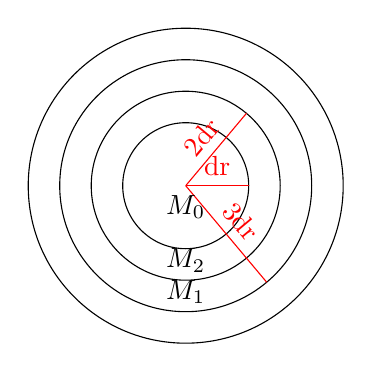
\begin{tikzpicture}[scale=0.8]
		\draw (2.5,2.5) circle(1);
		\draw (2.5,2.5) circle(1.5);
		\draw (2.5,2.5) circle(2);
		\draw (2.5,2.5) circle(2.5);
		\draw[red] (2.5,2.5) -- (3.5,2.5) node[midway, above] {$\mathrm{dr}$};
		\draw[red] (2.5,2.5) -- ++(50:1.5) node[sloped, above, midway] {$2 \mathrm{dr}$};
		\draw[red] (2.5,2.5) -- ++(-50:2) node[sloped, above, midway] {$3 \mathrm{dr}$};
		\draw (2.5,2.5) node[below]{$M_0$};
		\draw (2.5,1.15) node[below]{$M_1$};
		\draw (2.5,1.65) node[below]{$M_2$};
	\end{tikzpicture}
}
\parpic{
	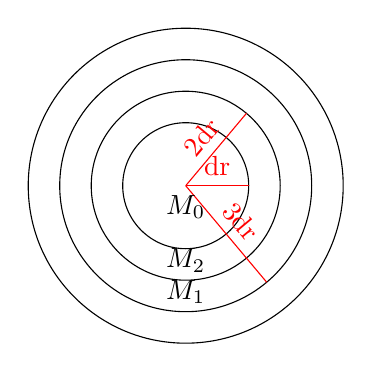
\begin{tikzpicture}[scale=0.8]
		\draw (2.5,2.5) circle(1);
		\draw (2.5,2.5) circle(1.5);
		\draw (2.5,2.5) circle(2);
		\draw (2.5,2.5) circle(2.5);
		\draw[red] (2.5,2.5) -- (3.5,2.5) node[midway, above] {$\mathrm{dr}$};
		\draw[red] (2.5,2.5) -- ++(50:1.5) node[sloped, above, midway] {$2 \mathrm{dr}$};
		\draw[red] (2.5,2.5) -- ++(-50:2) node[sloped, above, midway] {$3 \mathrm{dr}$};
		\draw (2.5,2.5) node[below]{$M_0$};
		\draw (2.5,1.15) node[below]{$M_1$};
		\draw (2.5,1.65) node[below]{$M_2$};
	\end{tikzpicture}
}\newcaption{Découpage de l'amas généré\label{schema::bin}}
\end{comment}
\begin{wrapfigure}{l}{0.28\textwidth}
%	\begin{center}
		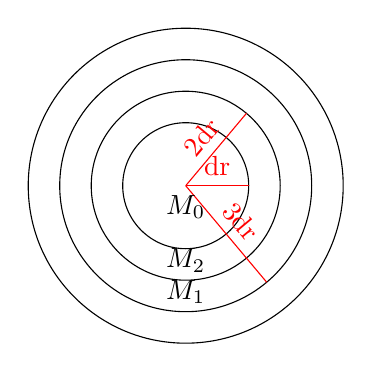
\begin{tikzpicture}[scale=0.8]
			\draw (2.5,2.5) circle(1);
			\draw (2.5,2.5) circle(1.5);
			\draw (2.5,2.5) circle(2);
			\draw (2.5,2.5) circle(2.5);
			\draw[red] (2.5,2.5) -- (3.5,2.5) node[midway, above] {$\mathrm{dr}$};
			\draw[red] (2.5,2.5) -- ++(50:1.5) node[sloped, above, midway] {$2 \mathrm{dr}$};
			\draw[red] (2.5,2.5) -- ++(-50:2) node[sloped, above, midway] {$3 \mathrm{dr}$};
			\draw (2.5,2.5) node[below]{$M_0$};
			\draw (2.5,1.15) node[below]{$M_1$};
			\draw (2.5,1.65) node[below]{$M_2$};
		\end{tikzpicture}
%	\end{center}
	\caption{Découpage de l'amas généré\label{schema::bin}}
\end{wrapfigure}
Le premier histogramme que nous générerons sera celui représentant
la masse en fonction du rayon. Notre objet étant sphérique, nous allons le
découper en intervalles de taille $\mathrm{dr}$ comme sur le schéma ci-contre. La fonction
de masse représente la masse se trouvant dans l'intervalle \mbox{$\left[0; j \mathrm{dr}\right]$}.
Pour la calculer, nous comptons le nombre de particules dans chaque chaque coquille sphérique de largeur $dr$ (~bin~), puis,
après avoir multiplié par la masse d'un particule, nous sommons, pour le bin
$j$, tous les bins inférieurs.

En même temps que nous calculons la fonction de masse, nous pouvons calculer la
densité en divisant la masse dans un bin par le volume du bin :
\begin{align}
	\rho_\mathrm{bin} &= \dfrac{M_\mathrm{bin}}{V_\mathrm{bin}} \notag \\
	\rho_i = \rho\( (i+1) \mathrm{dr}\) &= \dfrac{M_{\mathrm{bin}\ i}}{V_{\mathrm{bin}\ i}} \\
		&= \dfrac{M_{\mathrm{bin}\ i}}{\frac{4}{3}\pi ( (i+1)\mathrm{dr})^3 - \frac{4}{3}\pi ( i\mathrm{dr})^3} \notag \\
		&= \dfrac{3 M_{\mathrm{bin}\ i}}{4 \pi \mathrm{dr}^3 \left[ (i+1)^3 - i^3\right]} \notag \\
		&= \dfrac{3 M_{\mathrm{bin}\ i}}{4 \pi \mathrm{dr}^3 \left[ 3 i^2 + 3 i + 1\right]} \\
		&= \dfrac{3 \(M_i - M_{i-1}\)}{4 \pi \mathrm{dr}^3 \left[ 3 i^2 + 3 i + 1\right]}
\end{align}
avec $M_{-1} = 0$.

La densité obtenue et celle prévue par la résolution numérique sont très proche,
comme le montre le graphique~\ref{Comp_gene-theo}.
\begin{figure}[h!]
	\centering 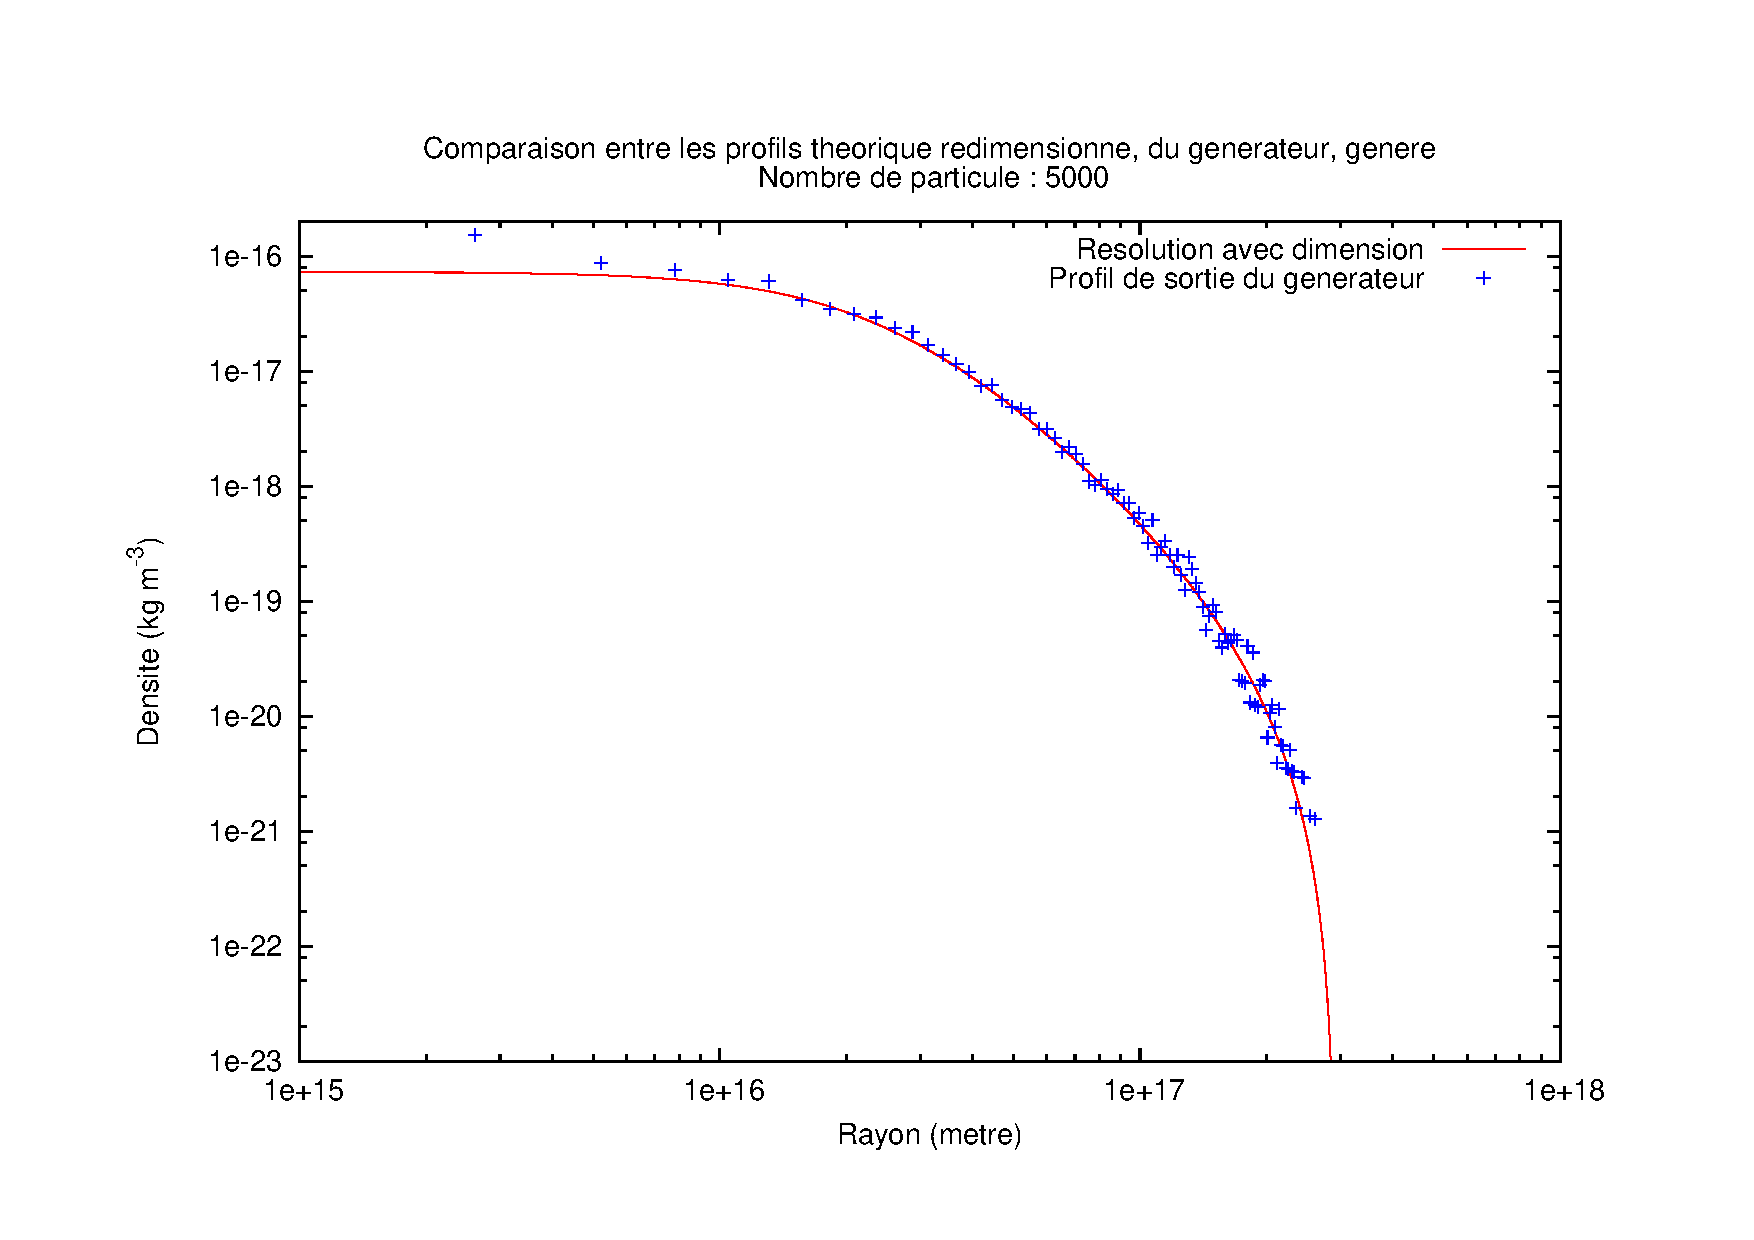
\includegraphics[scale=0.5]{graphe/Comp_dens_gene-theo_5000.pdf}
	\caption{Comparaison entre la résolution numérique et la densité donnée par le générateur\label{Comp_gene-theo}}
\end{figure}

\subsection{Énergie et potentiel}

La partie la plus complexe de la vérification est le calcul de l'énergie. Deux
choix s'offrent à nous :
\begin{itemize}
	\item la méthode force brute : nous calculons l'énergie totale en utilisant
		l'expression newtonienne du potentiel :
		$$
			E_{tot} = \frac{1}{2}\sum_{i = 1}^{N} m_i v_i^2 - G \sum_{i = 1}^{N} \sum_{j < i} \dfrac{m_i m_j}{|| r_i - r_j ||}
		$$
		avec $N$ le nombre de particule Le problème de cette méthode est qu'elle nécessite $N^2$
	opérations et n'est donc pas intéressante lorsque nous travaillons avec un grand
	nombre de particules. De plus, si deux particules sont très proche,
	l'énergie potentielle va diverger.
	\item la réflexion : nous avons déjà calculé la densité, et nous avons
		la fonction de masse, nous avons tout ce qu'il nous faut pour
		avoir le potentiel à partir de l'équation de \textsc{Poisson}.
\end{itemize}

Nous allons calculer le potentiel en résolvant l'équation de \textsc{Poisson}. Voyons
comment la résoudre avec ce que nous avons.
\begin{align}
	\Delta\psi &= \frac{1}{r^2}\dfrac{d}{dr}\( r^2 \dfrac{d \psi(r)}{dr} \) = 4\pi G \rho(r) \notag \\
	r^2 \dfrac{d \psi(r)}{dr} &= 4\pi G \int_0^r \rho(r) r^2 dr = G M(r) \notag \\
	\intertext{La densité est une fonction continue par morceau, nous pouvons donc écrire :}
	M(r)    &= 4\pi \int_0^r \rho(r) r^2 dr \notag \\
		&= 4\pi \sum_{j = 0}^{i - 1} \int_{j \mathrm{dr}}^{(j+1)\mathrm{dr}} \rho_j r^2 dr + 4\pi \int_{r_{i-1}}^r r^2 dr \text{, $r\in\left[ r_{i - 1}; r_i \right]$} \notag \\
		&= 4\pi \sum_{j = 0}^{i - 1} \rho_j \left[ \dfrac{r^3}{3} \right|_{j \mathrm{dr}}^{(j+1)\mathrm{dr}} + 4\pi\rho_i\left[\dfrac{r^3}{3}\right|_{r_{i - 1}}^{r} \notag \\
		&= 4\pi \sum_{j = 0}^{i - 1} \dfrac{\rho_j}{3} \mathrm{dr}^3 \( (j+1)^3 - j^3)\) + \dfrac{4\pi \rho_i}{3} \(r^3 - i^3\mathrm{dr}^3\) \notag \\
		&= M(r_{i-1}) + \dfrac{4\pi \rho_i}{3} \(r^3 - i^3\mathrm{dr}^3\) \notag \\
	\intertext{Ceci nous permet alors d'écrire le potentiel :}
	\psi(r) - \psi(0) &= G \int_0^r \dfrac{M(r)}{r^2} dr \notag \\
	\psi\(r_i\) - \psi(0) &= G \sum_{j = 0}^{i} \left\{\int_{j \mathrm{dr}}^{(j+1)\mathrm{dr}} \dfrac{M(r_{j-1})}{r^2} + \dfrac{4\pi \rho_j}{3 r^2} \(r^3 - j^3\mathrm{dr}^3\) dr\right\} \notag \\
	\intertext{avec $ r_i = (i+1) \mathrm{dr} $}
	\psi(r_i) - \psi(0) &= G \sum_{j = 0}^{i} \left\{M_{j-1} \left[ \dfrac{-1}{r}\right|_{j \mathrm{dr}}^{(j+1)\mathrm{dr}} + \dfrac{4\pi \rho_j}{3} \( \left[ \dfrac{r^2}{2} \right|_{j \mathrm{dr}}^{(j+1)\mathrm{dr}} - j^3\mathrm{dr}^3 \left[ \dfrac{-1}{r}\right|_{j \mathrm{dr}}^{(j+1)\mathrm{dr}} \)\right\} \notag \\
			    &=  G \sum_{j = 0}^{i} \left\{\dfrac{1}{j ( j + 1 ) \mathrm{dr}} \( M_{j - 1} - \dfrac{4\pi \rho_j}{3}j^3\mathrm{dr}^3 \) + \dfrac{4\pi \rho_j}{6}\( 2 j + 1 \)\mathrm{dr}^2\right\}
%			    &=  G \sum_{j = 0}^{i} \left\{\dfrac{1}{j ( j + 1 ) \mathrm{dr}} \( 4\pi \sum_{z = 0}^{j - 1}\( \dfrac{\rho_z}{3} \mathrm{dr}^3 \( (z+1)^3 - z^3\)\) - \dfrac{4\pi \rho_j}{3}j^3\mathrm{dr}^3 \) + \dfrac{4\pi \rho_j}{6}\( 2 j + 1 \)\mathrm{dr}^2\right\} \notag \\
%			    &=  G \sum_{j = 0}^{i} \left\{\dfrac{1}{j ( j + 1 ) \mathrm{dr}} \( 4\pi \sum_{z = 0}^{j - 1}\( \dfrac{\rho_z}{3} \mathrm{dr}^3 \( 3 z^2 + 3 z + 1\)\) - \dfrac{4\pi \rho_j}{3}j^3\mathrm{dr}^3 \) + \dfrac{4\pi \rho_j}{6}\( 2 j + 1 \)\mathrm{dr}^2\right\}
	\intertext{Pour le bin central $j = 0$, nous avons :}
	\psi(dr) - \psi(0)  &=  G \dfrac{4\pi \rho_0}{6}\mathrm{dr}^2
\end{align}

Pour obtenir la constante $\psi(0)$, nous allons nous servir des conditions sur le bord du système. En effet, nous avons vu plus haut que :
\begin{align}
	\psi_\mathrm{max} = \psi(R) &= - \frac{G M}{R} \\
	\intertext{Donc :}
	\psi(R) + \psi(0) - \psi(0) &= - \frac{G M}{R} \\
	\psi(0) &= - \frac{G M}{R} - \(\psi(R) - \psi(0)\) \\
	\psi(0) &= \frac{E_l}{m} - \(\psi(R) - \psi(0)\)
\end{align}

Le graphique~\ref{potentiel_5000} nous montre le potentiel théorique et le potentiel calculé par cette méthode.

\begin{figure}[h!]
	\centering 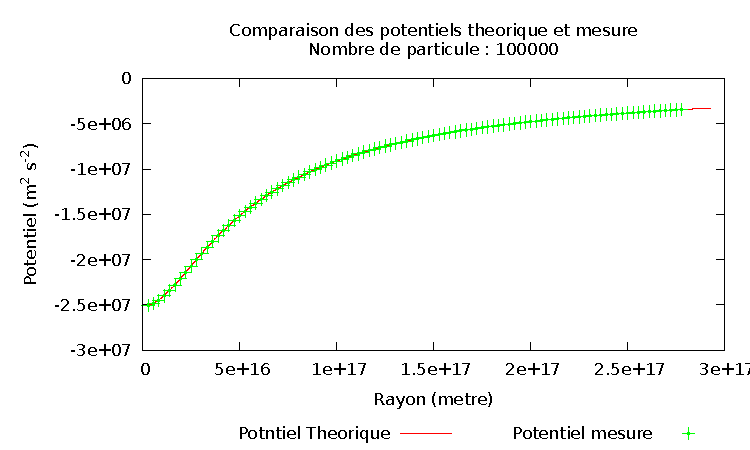
\includegraphics{graphe/Potentiel_ci-100000.pdf}
	\caption{Comparaison entre la résolution numérique et le potentiel donné par le générateur\label{potentiel_5000}}
\end{figure}

%Nous pouvons maintenant calculer la différence de potentiel entre le centre de l'amas et un rayon $r_i = (i+1)\mathrm{dr}$, mais nous ne connaissons pas
%$\psi(0)$ qui nous permettrait de remonter au potentiel qui nous intéresse pour le calcul de l'énergie. L'une des solutions évoqué, et utilisé, est
%d'appliquer le théorème du Viriel :
%\begin{align}
%	2Ec + Ep &=0 \\
%	-\sum_{i = 1}^N m_i\psi(r_i) &= -2 E_c \\
%	\sum_{i = 1}^N m_i\(\psi(r_i) + \psi(0) - \psi(0)\) &= 2 E_c \\
%	M_{tot}\psi(0) &= 2 E_c - \sum_{i = 1}^N m_i \(\psi(r_i) - \psi(0)\)
%\end{align}

\subsection{Forme de l'amas}

Maintenant que la densité et le potentiel de l'amas généré ont été vérifiés, il faut aussi vérifier que l'amas ne change pas de forme : nous générons un amas sphérique, nous devons~\footnote{il a en effet été montré qu'un \textsc{King}
non collisionnel est stable~\cite{JPerez96}} conserver un amas sphérique après l'avoir
fait évoluer. Pour vérifier que la forme de l'amas ne change pas, nous allons regarder comment évoluent les axes principaux d'inertie. Pour ce faire, nous allons calculer les valeurs propres de la matrice d'inertie :
\begin{align}
	\mathfrak{I} &= \(\begin{array}{ccc}
				\int \(y^2 + z^2\) dm & - \int xy dm & - \int xz dm \\
				-\int xy dm & \int \(x^2 + z^2\) dm & - \int yz dm \\
				-\int xz dm & -\int yz dm & \int \(x^2 + y^2\) dm
			\end{array}\) \\
		     &= \(\begin{array}{ccc}
				A & - D & - E \\
				-D & B & - F \\
				-E & -F & C
			\end{array}\)\notag
	\intertext{L'équation aux valeurs propres va alors s'écrire :}
	\left|\mathfrak{I} - \lambda \mathbb{I}\right|  &= \(A - \lambda\)\left[\(B-\lambda\)\( C-\lambda\) - F^2\right] + D \(-D\(C-\lambda\) - F E\) - E \left[ D F + E\(B - \lambda\)\right] \notag %\\
%						0	&= \(A - \lambda\)\(B-\lambda\)\( C-\lambda\) - \(A - \lambda\) F^2 - \(C-\lambda\) D^2 - \(B - \lambda\) E^2 \notag\\
%						0	&= \(A - \lambda\)\(BC - \lambda\(B + C\) + \lambda^2\) - \(A - \lambda\) F^2 - \(C-\lambda\) D^2 - \(B - \lambda\) E^2 \notag\\
%						0	&= A B C - \lambda A \(B+C\) + A \lambda^2 - B C \lambda + \lambda^2\(B+C\) - \lambda^3 - \(A - \lambda\) F^2 - \(C-\lambda\) D^2 - \(B - \lambda\) E^2 \notag\\
%						0	&= -\lambda^3 + \lambda^2\(A + B + C\) - \lambda\( A \(B+C\) + BC - F^2 - D^2 - E^2\) + A B C - A F^2 - C D^2 - B E^2 \notag
\end{align}
polynôme d'ordre 3 que l'on résout avec la méthode de \textsc{Cardan}. %~\footnote{\url{http://fr.wikipedia.org/wiki/Méthode_de_Cardan}}.

Une fois ces valeurs propres obtenues, si elles existent, nous traçons l'évolution des rapports $\lambda_1 / \lambda_2$ et $\lambda_3 / \lambda_2$, les valeurs propres étant numérotées dans l'ordre décroissant
\mbox{$\lambda_1 > \lambda_2 > \lambda_3$}.
